\documentclass[12pt]{article}

\topmargin 0.0cm 
\oddsidemargin 0.0in 
\evensidemargin0.0in
\textheight 22cm 
\textwidth  17cm 
\headheight 0in 
\headsep 0in
\parindent0in

\usepackage{amsmath}
\usepackage{amsfonts}
\usepackage{amssymb}
\usepackage{graphicx}
\usepackage{tikz}
\usepackage{amssymb}
\usepackage{circuitikz}
\usepackage{setspace}
\usepackage{subcaption}
\usepackage{multirow}
\usepackage{listings}
\usepackage{xcolor}
\usepackage{pdfpages}
\doublespacing
\lstset{
    language=Verilog,                % 设置语言
    basicstyle=\ttfamily\small,      % 设置等宽字体
    keywordstyle=\color{blue},       % 关键字颜色
    commentstyle=\color{gray},       % 注释颜色
    stringstyle=\color{orange},      % 字符串颜色
    numbers=left,                    % 行号显示在左侧
    numberstyle=\tiny\color{gray},   % 行号字体
    breaklines=true,                 % 自动换行
    frame=single,                    % 给代码加框
    captionpos=b                     % 标题放在下方
}





\begin{document}
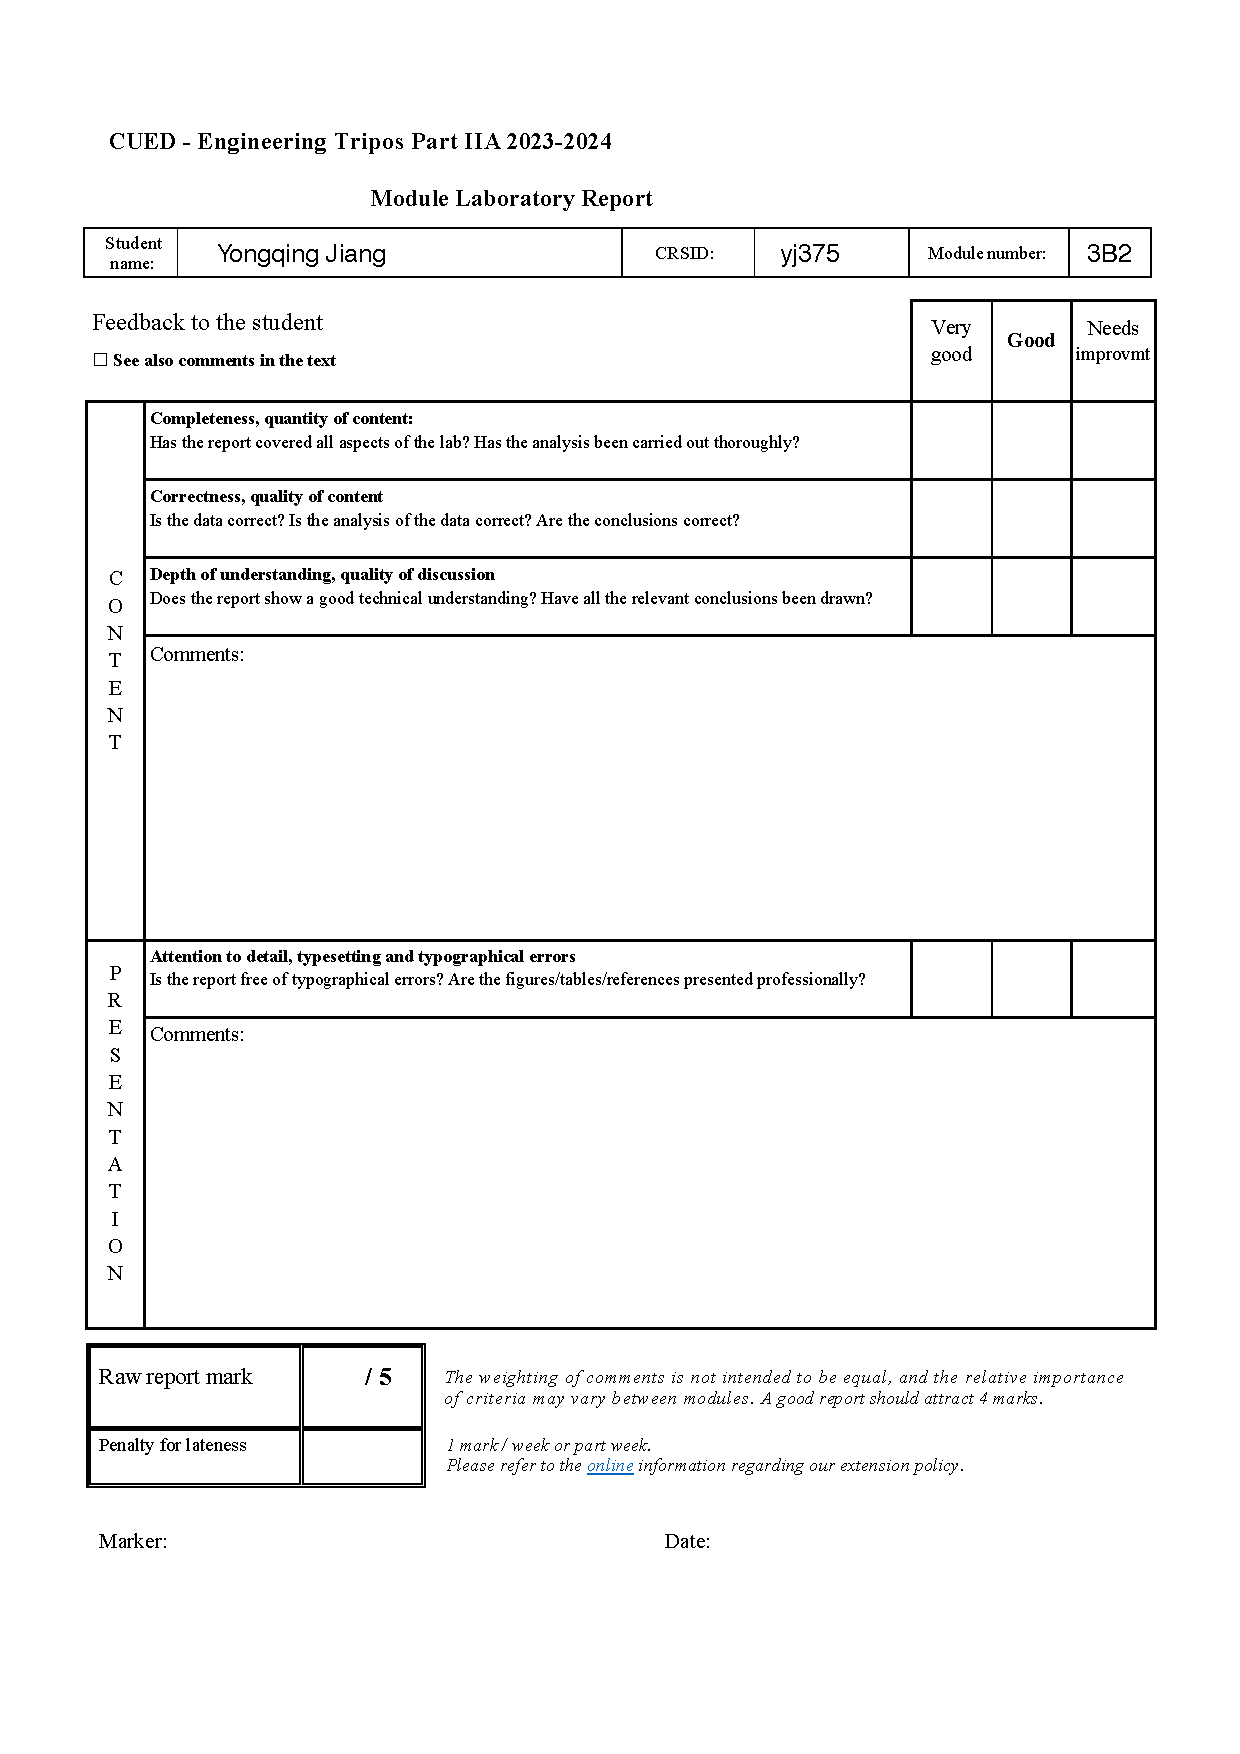
\includepdf{3B2 cover sheet.pdf}
%\hspace{1cm}

\begin{center}
\Large{\bf CAMBRIDGE UNIVERSITY ENGINEERING DEPARTMENT}
\end{center}

\vskip 0.5cm

\begin{center}
\large{\bf Part IIA Laboratory Report}
\end{center}

\vskip 0.5cm
\begin{center}
\fbox{\rule[0.0cm]{0cm}{1.0cm}
 \large{\bf 3B2 FPGA Programming and Testing}\rule[-0.75cm]{0cm}{1.0cm} }
\end{center}

\vskip 0.5cm

\begin{center}

Name: Yongqing Jiang \\
\vskip 0.2cm
CRSid: yj375  \\
\vskip 0.2cm
 College: Peterhouse \\
\vskip 0.2cm

Date of Experiment: Feb. 2026

\end{center}

\vskip 1cm

\section{Introduction}
This lab activity attempts to implement a logic function
that was shown on the lecture on a DE1-SoC development 
board, which presents a hardware design platform 
built on Altrea Cyclone V FPGA.
The provided verilog code is compiled and uploaded to the development
board via Quartus Prime, in which pin assessment is available. The 
FPGA board was tested under different user input. Lastly, 
some improvements 
are made to adapt to real-world situations.

\section{Problem Description and Design}
This design aims to model a controller of pedestrian light-controlled
crossing, as shown by Figure \ref{fig:plc}.
\begin{figure}[htbp]
    \centering
    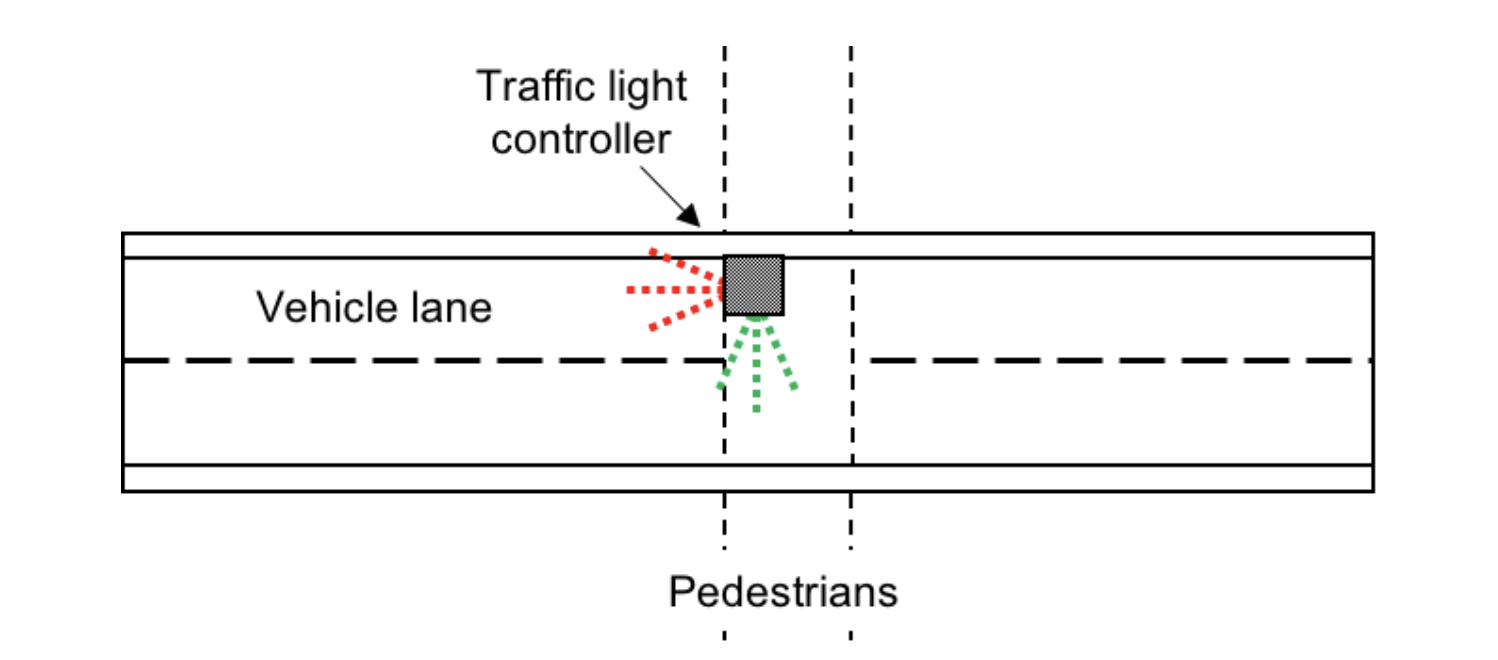
\includegraphics[width=0.8\textwidth]{fig1.png} 
    \caption{Pedestrian light-controlled crossing}
    \label{fig:plc}
\end{figure}

In this scenario, the traffic light controller controls 
2 lights: pedestrian light and vehicle light. The vehicle
light has three valid states: RED, YELLOW, and GREEN, while
the pedestrian light has two valide states: RED, and GREEN.

The external inputs include REQUEST from pedestrian-pressed
button, RESET to ensure the robustness of the system, and 
two timers T5 and T10 to enable internal time recording. 

The requirement of the traffic light control system is given as:
\begin{enumerate}
    \item The initial state is vehicle GREEN and pedestrian RED;
    \item It can only change state by demand, i.e. a pedestrian request or reset;
    \item After a request is made, the following 3-state sequence needs to be implemented:
    \begin{itemize}
        \item It starts by turning vehicle to YELLOW for 5 seconds;
        \item Then it turns vehicle to RED and pedestrian to GREEN at the same time, both for
        10 seconds;
        \item Then it returns to the initial state.
    \end{itemize}
    \item A reset command returns the system to its initial state.
\end{enumerate}
The state transition diagram is shown by Figure \ref{fig:statediag}.
It is important to note that the problem is reduced to have only
3 states labelled by the current vehicle light. This is 
because the pedestrian light is dependent on vehicle light.
\begin{figure}[htbp]
    \centering
    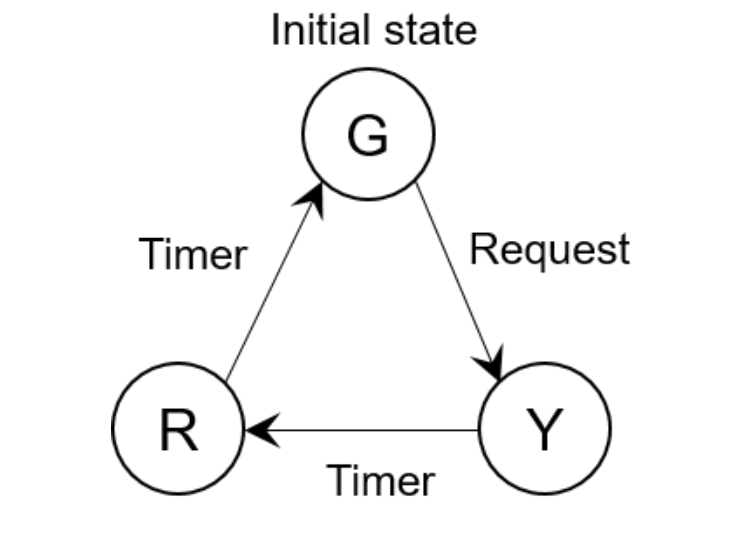
\includegraphics[width=0.5\textwidth]{fig2.png} 
    \caption{State diagram of the problem}
    \label{fig:statediag}
\end{figure}

From the state diagram, a state table can be constructed as
shown in Table \ref{tab:statetable}.


\begin{table}[htbp]
    \centering
    \renewcommand{\arraystretch}{1.2} 
    \begin{tabular}{|c|c|c|c|c|c|c|c|c|c|}
    \hline
    \textbf{State} & \multicolumn{4}{c|}{\textbf{Next state}} & \multicolumn{3}{c|}{\textbf{Vehicle lights}} & \multicolumn{2}{c|}{\textbf{Pedestrian}} \\ 
     & \multicolumn{4}{c|}{} & \multicolumn{3}{c|}{} & \multicolumn{2}{c|}{\textbf{lights}} \\ \cline{2-10}
     & Reset & Request & 5 s & 10 s & GREEN & YELLOW & RED & GREEN & RED \\ \hline
    G & G & Y & & & 1 & 0 & 0 & 0 & 1 \\ \hline
    Y & G & & R & & 0 & 1 & 0 & 0 & 1 \\ \hline
    R & G & & & G & 0 & 0 & 1 & 1 & 0 \\ \hline
    \end{tabular}
    \caption{Traffic Light State Transition Table}
    \label{tab:statetable}
    \end{table}


\section{FPGA Implementation and Improvement}

The verilog code which could implement this design is provided
by the lab handout, which is included in the Appendix by 
Listing \ref{list:tlc}.

To implement this verilog code on hardware platform,
Quartus Prime is needed to compile and upload code 
to DE1-SoC.

The key steps in Quartus Prime include compiling verilog
code, pin assignment, configuring FPGA device, and 
uploading the code to FPGA.

After that, the designed circuit is tested by
pressing buttons that are assigned to give 
REQUEST and RESET signal, and observing the 
LED output that corresponds to 3 vehicle lights
and 2 pedestrian lights.

\begin{figure}[htbp]
    \centering
    \begin{subfigure}[b]{0.45\textwidth}
        \centering
        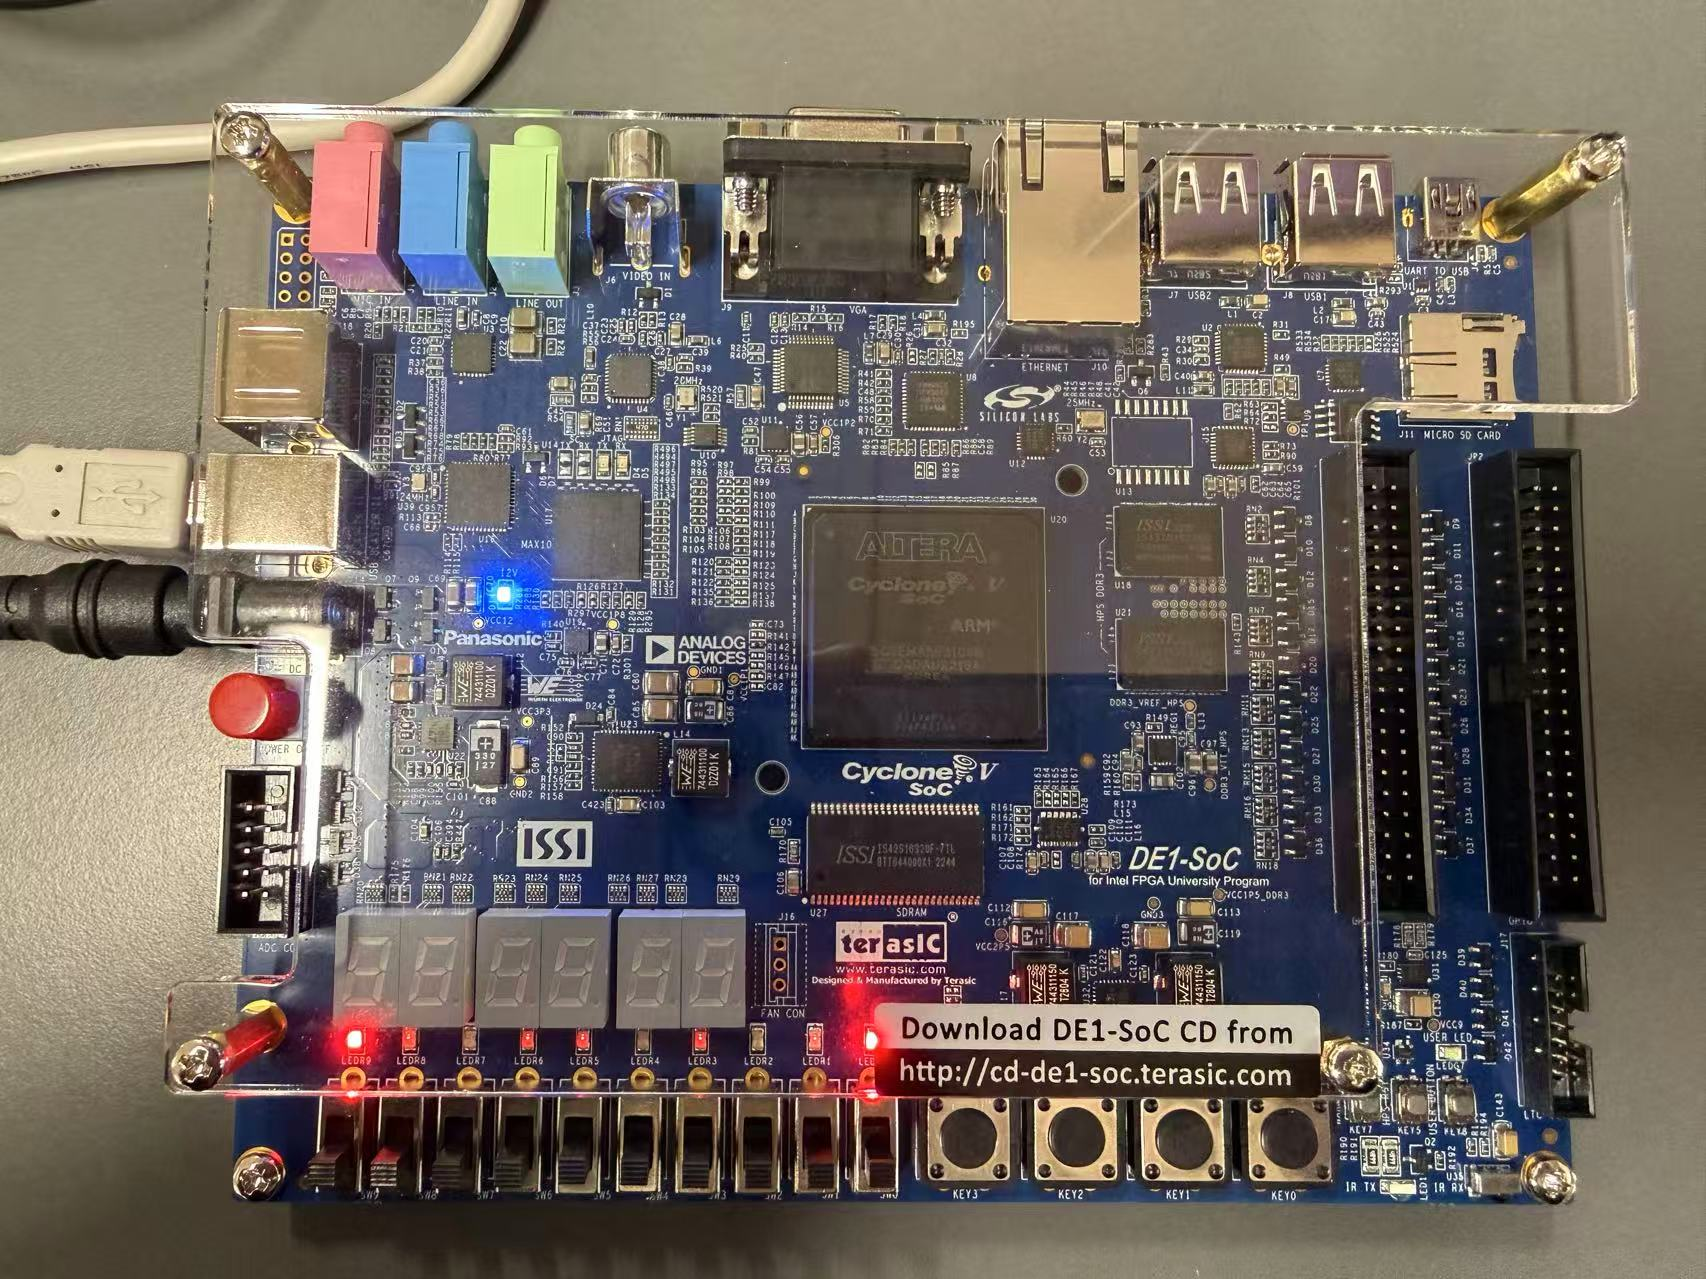
\includegraphics[width=\textwidth]{fpga1.jpg}
        \caption{State G: initial state}
        \label{fig:left}
    \end{subfigure}
    \hfill 
    \begin{subfigure}[b]{0.45\textwidth}
        \centering
        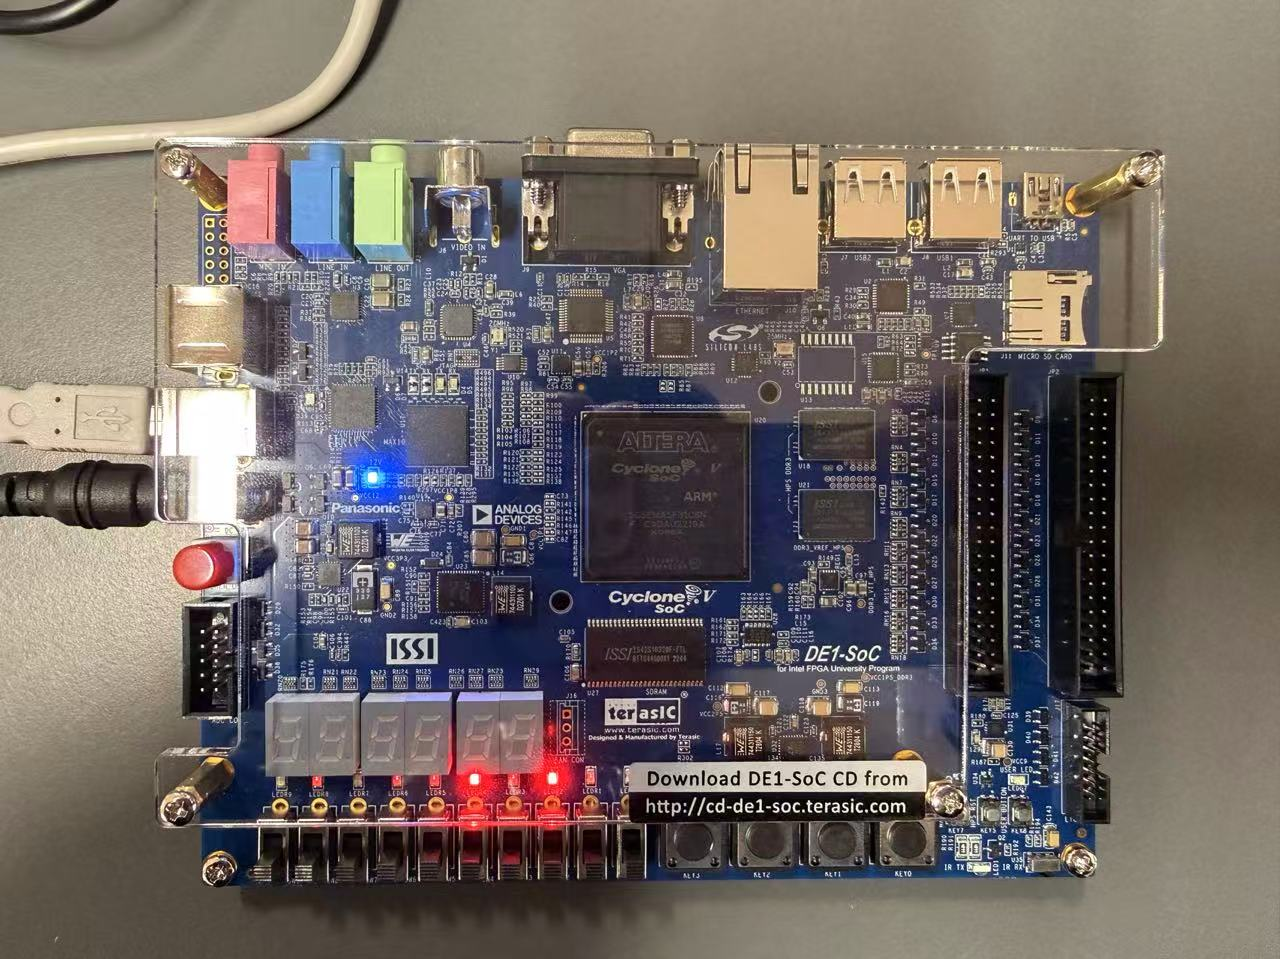
\includegraphics[width=\textwidth]{fpga2.jpg}
        \caption{State R: state 5s after REQUEST}
        \label{fig:right}
    \end{subfigure}
    
    \caption{Picture of FPGA board under operation}
    \label{fig:overall}
\end{figure}

Shown by Figure \ref{fig:overall}, 5 of 10 available LEDs
are assigned to 5 lights. The correspondence is:
\begin{enumerate}
    \item LED0: Pedestrian RED
    \item LED2: Pedestrian GREEN
    \item LED4: Vehicle RED
    \item LED7: Vehicle YELLOW
    \item LED9: Vehicle GREEN
\end{enumerate}
These lights are set to have space to each other
to simplify observation.

By pressing REQUEST and RESET buttons on different state,
the observation shows that the FPGA demonstrates the 
required design objective.



However, this design has a drawback. If the pedestrian
presses the button for multiple times, the Finite State Machine
would always initiate and it would never stays at State G.
Which means that the vehicle light never turns green, blocking
the traffic.

This could be improved by slight modification on 
the condition of transition from State G to Y.
The original code from line 18 to 
23 is modified as shown by Listing \ref{list:mod}.


\begin{lstlisting}[caption={modified state transition},label={list:mod}]
    reg req_latch;
    G: begin
		if (req == 1'b0) begin
			req_latch <= 1'b1;
		end
		if (count < 29'd500000000 ) begin
			count <= count + 29'd1;
		end 
		if ((count >= 29'd500000000) && ((req == 1'b0)||(req_latch == 1'b1))) begin
			state <= Y;
			count <= 29'd0;
			req_latch <= 1'b0;
		end
    Y: begin
        ...
    
\end{lstlisting}
In this design, an intermediate 1-bit register 
\verb|req_latch| is created. This acts as a 
temporary storage of REQUEST signals. 
No matter how many times the button is pressed, 
the latch keeps to be 1 until state transition happens.

State G is now kept to last at least 10 seconds before it 
transits to Y. When it passes more than 10 seconds and either a 
REQUEST button is pressed or there is a stored REQUEST signal, 
G transits to Y and \verb|req_latch| is initialized to 0.

As a result, if the button is pressed for multiple times, 
the vehicle green light will be ON for at least 10 seconds
before it turns yellow, avoiding the case that 
traffic is blocked due to multiple pedestrian press. 

However, this implies that even though there is no vehicle on 
the lane, the pedestrian will still needs to wait
for 10 seconds after pressing the button, if the pedestrian
unfortunately arrives right after the pedestrian light 
turning red. 

The expected wait time is definitely lower
than 10 seconds, since the pedestrian could arrive 
anytime, and it is independent of the state transition
of the traffic light controller. If the pedestrian
arrives more than 10 seconds after the vehicle light 
turning green, no wait time is needed under 
this situation. The evaluation of expected wait time
requires extra statistical modelling.

\section{Conclusion}   

In this laboratory activity, a pedestrian 
light-controlled crossing system was 
successfully implemented and verified on 
the DE1-SoC FPGA platform. 
By applying Finite State Machine 
design principles, the required transition 
logic between vehicle 
and pedestrian lights was 
established and validated through hardware 
testing. The use of Quartus Prime for pin 
assignment and FPGA configuration ensured 
that the digital design correctly interfaced 
with physical peripherals, such as push-buttons 
for inputs and LEDs for status display.


Beyond the basic implementation, 
a significant limitation regarding 
traffic flow efficiency was identified 
in the original design. By introducing a 
 \verb|req_latch| mechanism and 
a minimum duration constraint for the 
vehicle Green state, the system was made 
more robust against frequent pedestrian 
requests. This improvement prevents
potential traffic congestion while 
maintaining system operation. 
Although this introduces a deterministic 
waiting period for pedestrians, it 
represents a necessary trade-off in 
real-world infrastructure design. 
Future enhancements could involve more 
sophisticated sensor integration or 
machine-learning based control of 
traffic light states.




\section{Appendix}
Original code provided by lab handout:

\begin{lstlisting}[caption={original implementation of traffic light controller },label={list:tlc}]
    module tlc (
        input wire clk,
        input wire request,
        input wire reset,
        output reg [4:0] \output
    );
        localparam G = 2'd0;
        localparam Y = 2'd1;
        localparam R = 2'd2;
        reg [1:0] state;
        reg [28:0] count;
        always @(posedge clk or negedge reset) begin
            if (!reset) begin
                state <= G;
                count <= 29'd0;
            end else begin
                case (state)
                    G: begin
                        if (request == 1'b0) begin
                            state <= Y;
                            count <= 29'd0;
                        end
                    end
                    Y: begin
                        if (count == 29'd250000000) begin
                            state <= R;
                            count <= 29'd0;
                        end else begin
                            count <= count + 29'd1;
                        end
                    end
                    R: begin
                        if (count == 29'd500000000) begin
                            state <= G;
                            count <= 29'd0;
                        end else begin
                            count <= count + 29'd1;
                        end
                    end
                    default: begin
                        state <= G;
                        count <= 29'd0;
                    end
                endcase
            end
        end
        always @(*) begin
            case (state)
                G: \output = 5'b10001;
                Y: \output = 5'b01001;
                R: \output = 5'b00110;
                default: \output = 5'b10001;
            endcase
        end
    endmodule
\end{lstlisting}
\end{document}